

%!TEX root = ./main.tex
%** Results.tex: What were the results achieved including an evaluation
\chapter{Evaluation and Results\label{chapter:results}}

\section{Evaluation}

In order to evaluate the effect of server socket based traffic preselection, three known events were analyzed with the old port-based heuristic of FACT as well as with the new server socket based approach. Then, both results are compared and the effect of the traffic preselection on the noise of the results is qualitatively discussed.

\subsection{Partitioned Internet Exchange Point}
% PAM-PAPER: On March 23, 2010: After scheduled maintenance by AMS-IX, SWITCH’s connection to that exchange point came back with only partial connectivity. Some next-hops learned via the route servers weren’t reachable, creating black holes. The next morning, several customers complained about external services being unreachable. Overall, it took more than four hours until the problem was finally solved by resetting a port.

The IXP \citet{AMS-IX}(AMS-IX) performed on March 23, 2010 a scheduled maintenance. When its connection to \citet{switch} came back, there was only a partial connectivity through this IXP, since some next-hops learned via their route servers were not properly reachable, thus traffic towards these networks are black-holed.\citep{SchatzmannPAM2011}

In consequence, several internal clients of the \citet{switch} network were complaining about unreachable external services on the next morning. Using classical debugging tools, it took more than four hours for fixing the problem by resetting a port.\citep{SchatzmannPAM2011}

\subsubsection{Heuristic Approach}
This event is well visible by the classical FACT, since there are quite a large number of affected users thus favoring the user aggregation approach of detecting relevant events. Figure \ref{fig:AMS_IX_FACT_REF} shows the number of unreachable BGP prefixes over time separated by the number of affected internal clients. As previously outlined the user aggregation approach tries to prioritize severe events by determining the number of affected internal users. Hence, the severity of the events is indicated by the color of the unreachable prefixes in figure \ref{fig:AMS_IX_FACT_REF}. To be precise, the pink prefixes denotes the unreachable prefixes by at least 10 distinct internal clients, the blue respectively 5 distinct internal clients.

This specific IXP partitioning event is clearly visible in figure  \ref{fig:AMS_IX_FACT_REF} from 05.00 UTC to 08:15 UTC with almost 20 unreachable BGP prefixes affecting more than 10 internal clients and almost 200 unreachable BGP prefixes in total. However, as discussed in chapter \ref{Introduction}, those unreachable prefixes affecting only 1 client are not reliable observations, thus of limited interest representing a kind of observation noise of FACT.

\begin{figure}
	[hb] \centering 
	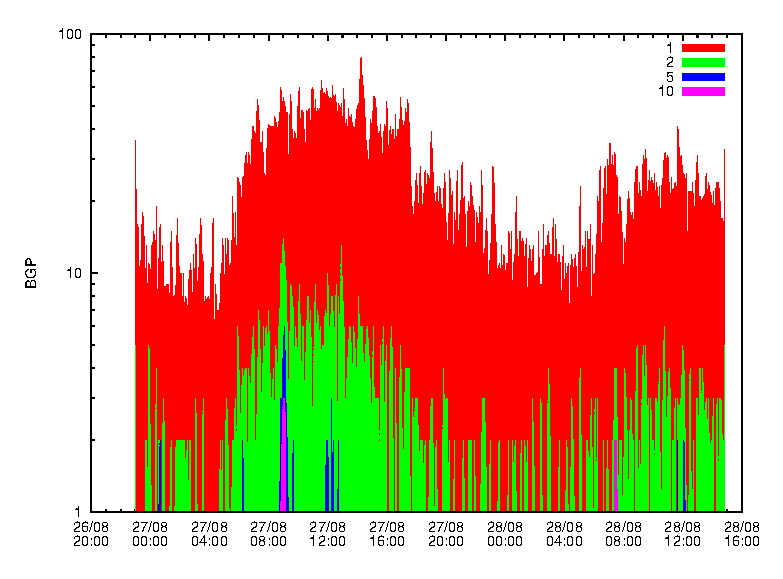
\includegraphics[width=\linewidth]{images/events/2010_03_25/bgp_log_port80_ref.eps}
	\caption{Unreachable BGP prefixes detected by the classical FACT traffic preselection based on the port-based heuristic.} 
	\label{fig:AMS_IX_FACT_REF} 
\end{figure}

\subsubsection{Server Socket Approach}
\begin{figure}
	[hb] \centering 
	\includegraphics[width=\linewidth]{images/events/2010_03_25/bgp_log_allPort80SES.eps}
	\caption{Unreachable BGP prefixes detected by the modified FACT traffic preselection based on all port 80 server sockets.} 
	\label{fig:AMS_IX_FACT_allSES80} 
\end{figure}


\subsubsection{Qualitative Comparison}


\subsection{Reverse path traffic black-holing by Tier-1}
% PAM-PAPER: On May 18, 2010, all services in an external /24 network were not accessible from SWITCH between 08:30 and 08:45. According to the oper- ators of SWITCH, this problem was most likely due to a tier-1 provider that black-holed parts of the reverse traffic towards SWITCH. Yet, at this time the operators could only speculate how many hosts and customers, or even other /24 networks were affected by this problem. Applying FACT we confirm that the reported /24 network is indeed reported as unreachable at around 08:30. Surprisingly, FACT reveals that the overall number of unreachable hosts and /24 networks has doubled compared to the time before 08:30 while the number of unresponsive BGP prefixes is increased by a factor of even 6, see Fig. 5(a). Moreover, the reported /24 network is not even in the top ten list of the most popular unresponsive networks. This suggests that the impact of this event has been more serious than previously believed.


\subsubsection{Heuristic Approach}

\subsubsection{Server Socket Approach}

\subsubsection{Qualitative Comparison}


\subsection{RIPE / DUKE BGP Experiments 2010-08-27}
% PAM-PAPER: On August 27, 2010, some parts of the Internet became disconnected for some 30 minutes due to an experiment with new BGP attributes by RIPE and Duke University [12]. FACT reveals that at around 08:45 the number of popular unresponsive /24 networks indeed doubled. According to Fig. 5(b), for some BGP prefixes more than 15 internal hosts failed to establish connectivity. Yet, overall our analysis reveals that the impact of this incident on SWITCH and its customers was quite limited compared to the public attention that this event obtained.

\subsubsection{Heuristic Approach}

\subsubsection{Server Socket Approach}

\subsubsection{Qualitative Comparison}


\section{Results}
